%
%
\chapter{Computation of the Static Susceptibility}
\label{appch: static susceptibility}
%
%
In this appendix, the static susceptibility $\chi_{\mt{JP}}(\omega=0)$ is explicitely calculated.
The temperature dependence of $\chi_{\mt{JP}}$ is expected to be non-existent, since momentum and current are not explicitly time dependent.
Using equation \eqref{eq:relation between C, Phi and chi}, the static susceptibility is directly proportional to the Kubo relaxation function \eqref{eq:Kubo relaxation function} at $t=0$.
%
\begin{align}
	\chi_{\mt{PJ}}(\omega = 0) = \Phi_{\mt{PJ}}(t = 0) = i \int\limits_{0}^{\infty} \dd{t'} \expval{\comm{\mt{P}_{j}(t')}{\mt{J}_{j}(0)}}
\end{align}
%
In the formula above, the limit $s\to0$ is dropped, since the integral is assumed to be convegent.
The spatial direction of P and J is signified by the index $j$.
The integral is transformed into Matsubara time $\tau = it$, firstly.
The Jacobi determinate is $-i$ and the integral's limits is set to $0$ and $\beta$.
Observing only the zeroth order in pertubation theory the static susceptibility is given by
%
\begin{align}
	\chi_{\mt{PJ}}(\omega = 0) = \int\limits_{0}^{\beta} \dd{\tau} \expval{\mathcal{T}_{\tau} \mt{P}_{j}(\tau) \mt{J}_{j}(0)}_{0}.
\end{align}
%
The momentum and current operators are denoted in equation \eqref{eq:momentum operator} and \eqref{eq:current operator}, respetivily.


In the investigated order only one pair of bosonic operators, \ie\, one propagator, and no interaction between the spin density waves and the electrons are observed.
Therefore the bosonic propagator yields always a disconnected diagram.
Furthermore pairing electrons of different Fermi sufaces isn't allowed, which means that the expactation value of mixed fermionic operators also yields disconnected diagrams.
Thus many diagrams of the investigated ones are disconnected, beside of two.
These two bubble diagrams are depicted in figure \ref{fig: static susceptibility}.
%
\begin{figure}
	\centering
	\includegraphics[width=0.8\textwidth]{static_susceptibility.eps}
	\caption{caption}
	\label{fig:static susceptibility}
\end{figure}
%
%
\begin{align}
	\chi_{\mt{PJ}}(\omega = 0) = 
		-\frac{1}{\hbar} 
		\int\limits_{0}^{\beta} \dd{\tau} 
		\int_{\vb{k}}
		\bigg[
			&\frac{k_{j}^{2}}{m_{1}}
			\expval{
				\mathcal{T}_{\tau}
				\Psi_{\mt{a}}^{\dag}(\vb{k},\tau)
				\Psi_{\mt{a}}(\vb{k},\tau)
				\Psi_{\mt{a}}^{\dag}(\vb{k},0)
				\Psi_{\mt{a}}(\vb{k},0)
			}_{0}
			\notag \\ +
			&\frac{k_{j}^{2}}{m_{2}}
			\expval{
				\mathcal{T}_{\tau}
				\Psi_{\mt{b}}^{\dag}(\vb{k},\tau)
				\Psi_{\mt{b}}(\vb{k},\tau)
				\Psi_{\mt{b}}^{\dag}(\vb{k},0)
				\Psi_{\mt{b}}(\vb{k},0)
			}_{0}
		\bigg]
\end{align}
%
\todo{Vielleicht noch etwas zu der delta-Distribution und so schreiben, damit klar is warum die Operatoren alle beim gleichen Impuls sind.}
The two expectation value of four fermionic operators can't be solved directly.
Wick's theorem offers the oppertunity to write these expectation values into a product of expectation values contained only two operators, which are nothing else free propagators.
Two contraction are possible for each expectation value in the investigated case above, where one of them vanishes, because the time argument of the contracted operator is the same.
%
\begin{align}
	\chi_{\mt{PJ}}(\omega = 0) &= 
		\frac{1}{\hbar} 
		\int\limits_{0}^{\beta} \dd{\tau} 
		\int_{\vb{k}} 
		k_{j}^{2}
		\bigg[
			\frac{1}{m_{1}}
			\mathcal{G}_{\mt{a}}^{(0)}(\vb{k},-\tau)
			\mathcal{G}_{\mt{a}}^{(0)}(\vb{k},\tau)
			+
			\frac{1}{m_{2}}
			\mathcal{G}_{\mt{b}}^{(0)}(\vb{k},-\tau)
			\mathcal{G}_{\mt{b}}^{(0)}(\vb{k},\tau)
		\bigg]
\end{align}
%
where the free fermionic propagator $\mathcal{G}_{\alpha}^{(0)}(\vb{k},\tau) = -\expval*{\mathcal{T}_{\tau} \Psi_{\alpha}(\vb{k},\tau) \Psi_{\alpha}^{\dag}(\vb{k},0)}$ with $\alpha \in \{\mt{a},\mt{b}\}$ is introduced.
The Green functions of electrons are transformed into the Matsubara frequency space, thus the only time dependence is at the exponential functions.
The $\tau$-integral yields a $\delta$-distrubution $\delta(\omega_{m} - \omega_{n})$ and then one sum over the Matsubara frequencies can be performed.
%
\begin{align}
	\chi_{\mt{PJ}}(\omega = 0) &= 
		\frac{1}{\hbar} 
		\int_{\vb{k}} 
		k_{j}^{2}
		\bigg[
			\frac{1}{m_{1}}
			S_{\mt{a}}(\omega_{n})
			+
			\frac{1}{m_{2}}
			S_{\mt{b}}(\omega_{n})
		\bigg],
\end{align}
%
where the Matsubara sum $S_{\alpha}(\omega_{n}) = \beta^{-1} \sum_{\omega_{n}} \mathcal{G}_{\alpha}^{(0)}(\vb{k},\omega_{n}) \mathcal{G}_{\alpha}^{(0)}(\vb{k},\omega_{n})$ is introduced.
The Matsubara theory exhibits that these kinds of sums can be evaluated by rewriting the sum as a contour integral in the complex plane, integrating over the Green function multiplied with the Fermi or Bose distribution caused by the nature of the Green function.
This transformation yields
%
\begin{align}
	S = \frac{1}{\beta} \sum\limits_{\omega_{n}} \mathcal{G}(\omega_{n}) = -\frac{1}{2\pi i} \oint_{\Gamma} \dd{z} n_{\mt{F}}(z) \mathcal{G}(z)
\end{align}
%
%
\begin{figure}
	\centering
	\includegraphics[width=0.8\textwidth]{contour_simple_poles.pdf}
	\caption{caption}
	\label{fig: contour simple poles}
\end{figure}
%
in the case of a fermionic Green function.
Thereby the contour is arbitrary.
The only important fact is that all singularities of the Green function has to be excluded of the contour.
Only the singularities of the distribution function are included in the contour.
The contour $\Gamma$ is expanded to infinity, where always the singularities of the Green function has to be excluded.
This procedure is depicted in figure \ref{fig: contour simple poles}.
The paths from infinity to the poles and back yield the same contribution beside the sign, why both cancel each outher.
The contour is therefore deformed to circles around the poles running clockwise and an infinite circle running counterclockwise.
The latter is zero, because the Green function is proportional to $\flatfrac{1}{z}$.
The electronic Green function is given by
%
\begin{align}
	\mathcal{G}_{\alpha}(\vb{k},\omega_{n}) = \frac{1}{i\omega_{n} - \epsilon_{\alpha}(\vb{k})},
\end{align}
%
where $\epsilon_{\alpha}(\vb{k})$  is the electron's dispersion relation with respect to the corresponding Fermi suface denoted with a and b (see equation \dots \todo{Link zu den Dispersionsrelationen}), has only simple poles in the complex plane, which means the function is continously in the whole complex plane.
Therefore the well known residuum theorem can be used to evaluate the contour integral.
%
\begin{align}
	\chi_{\mt{PJ}}(\omega = 0) &= 
		-\frac{1}{\hbar} 
		\int_{\vb{k}} 
		k_{j}^{2}
		\bigg[
			\frac{1}{m_{1}}
			\dv{n_{\mt{F}}(\epsilon_{\mt{a}}(\vb{k}))}{\epsilon_{\mt{a}}(\vb{k})}
			+
			\frac{1}{m_{2}}
			\dv{n_{\mt{F}}(\epsilon_{\mt{b}}(\vb{k}))}{\epsilon_{\mt{b}}(\vb{k})}
		\bigg]
\end{align}
%
The derivatives of the distribution function with respect to the dispersion relation appears because the singularity of the Green function at $z_{0} = \epsilon_{\alpha}(\vb{k})$ is a singularity of second order.
These two integrals are exactly solvable.
Therefore the inetegrals are transformed into polar coordinates.
The transformation rule is given by $(k_{x}, k_{y}) = (q\sqrt{2m_{1,2}}\cos(\phi), q\sqrt{2m_{2,1}}\sin(\phi))$, where two forms are used, because of the different dispersion relation.
The $k_{j}^{2}$-term originates the only angular dependence, which yields $\cos[2](\phi)$ or $\sin[2](\phi)$ for the $x$- or $y$-direction, respectivily.
Because the limits of the integral are $0$ and $2\pi$ the integral yields the same result in both cases.
The upper limit of the $q$-integral can be set to infity, because the integrand is decreased very fast to zero for large values of $q$.
%
\begin{align}
	\chi_{\mt{PJ}}(\omega = 0) = 
		\frac{8 \beta \pi}{(2\pi)^{2} \hbar} \sqrt{m_{1} m_{2}}
		\int\limits_{0}^{\infty} \dd{q}
		q^{3} \frac{e^{\beta(q^{2} - \mu)}}{(e^{\beta(q^{2} - \mu)} + 1)^{2}}
\end{align}
%
The obtained integral can be solved by substituting $x = \beta(q^{2} - \mu)$.
Thereby the first of the two integrals is evaluated with integration by parts
In the second integral the integrand is equal to the derivative of the Fermi distributation.
All in one the static susceptibility of P and J is given by
%
\begin{align}
	\chi_{\mt{PJ}}(\omega = 0) = \frac{\sqrt{m_{1} m_{2}}}{\pi \beta \hbar}\ln(e^{\beta \mu} + 1)
\end{align}
%
in first order pertubation theory. \todo{Heisst es nullte oder erste Ordnung St\"orungstheorie?}
In the case of $\mu \gg k_{\mt{B}} T$ the argument of the exponential function is very large.
Therefore the one is neglectable in the argument of the logarithm and $\ln(e^{\beta\mu} + 1) \approx \beta\mu$.
In the limit of small temperatures the susceptibility is given by
%
\begin{align}
	\chi_{\mt{PJ}}(\omega = 0) \to \frac{\mu \sqrt{m_{1} m_{2}}}{\pi \hbar} \qquad (T \to 0)
\end{align}
%
The static susceptibility between P and J is temperature independent in the limit of $\mu \gg k_{\mt{B}} T$, like exactly we have expected.